\input{../YKY-preamble.tex}

\title{Symmetric neural networks}
\author{YKY}

\begin{document}
\maketitle

\section{Convolutions have translational equivariance}

The following is quoted from Wikipedia:

\begin{tcolorbox}[breakable]
The convolution commutes with translations, meaning that

\begin{equation}
\tau_x (f * g) = (\tau_x f) * g = {f} * (\tau_x g)
\end{equation}
where $\tau_x f$ is the translation of the function $f$ by $x$ defined by:
\begin{equation}
(\tau_x f)(y) = f( y - x ) .
\end{equation}
If $f$ is a \textbf{Schwartz function}
	\footnote{Schwartz space is the function space of all functions whose derivatives are rapidly decreasing. This space has the important property that the Fourier transform is an automorphism on this space.}
, then $\tau_x f$ is the convolution with a translated Dirac delta function $\tau_x f = f * \tau_x \delta$.  So translation invariance of the convolution of Schwartz functions is a consequence of the associativity of convolution.

Furthermore, under certain conditions, \uline{convolution is the most general translation invariant operation}.  Informally speaking, the following holds:

\begin{list}{}{}
	\item Suppose that $S$ is a bounded linear operator acting on functions which commutes with translations: $S(\tau_x f) = \tau_x(S f)$ for all $x$. Then $S$ is given as convolution with a function (or distribution) $g S$; that is $S f = g S * f$.
\end{list}

Thus some translation invariant operations can be represented as convolution. Convolutions play an important role in the study of time-invariant systems, and especially LTI system theory. The representing function $g S$ is the impulse response of the transformation $S$.

A more precise version of the theorem quoted above requires specifying the class of functions on which the convolution is defined, and also requires assuming in addition that $S$ must be a continuous linear operator with respect to the appropriate topology. It is known, for instance, that every continuous translation invariant continuous linear operator on $L1$ is the convolution with a finite Borel measure. More generally, every continuous translation invariant continuous linear operator on $L_p$ for $1 \le p < \infty$ is the convolution with a tempered distribution whose Fourier transform is bounded.  To wit, they are all given by bounded Fourier multipliers.
\end{tcolorbox}

In 1989, Yann LeCun invented \textbf{convolutional} neural networks (ConvNets) which established the importance of this type of neural networks for \textbf{computer vision} (it seems to remain the dominant approach to this day).  For this he won the Turing Award recently.
\begin{equation}
\nonumber
\vcenter{\hbox{
\includegraphics[scale=0.25]{Yann-LeCun.jpg}}}
\end{equation}

In computer vision, translational invariance is obviously desirable.  The structure of ConvNets has translational invariance built-in, so it does not need to be learned, thus making learning more efficient.  This enabled the breakthrough in machine vision to surpass human level, around 2011.

\section{Structure of a standard neural network}

Recall that a neural network is constructed from \textbf{features}:
\begin{equation}
\vcenter{\hbox{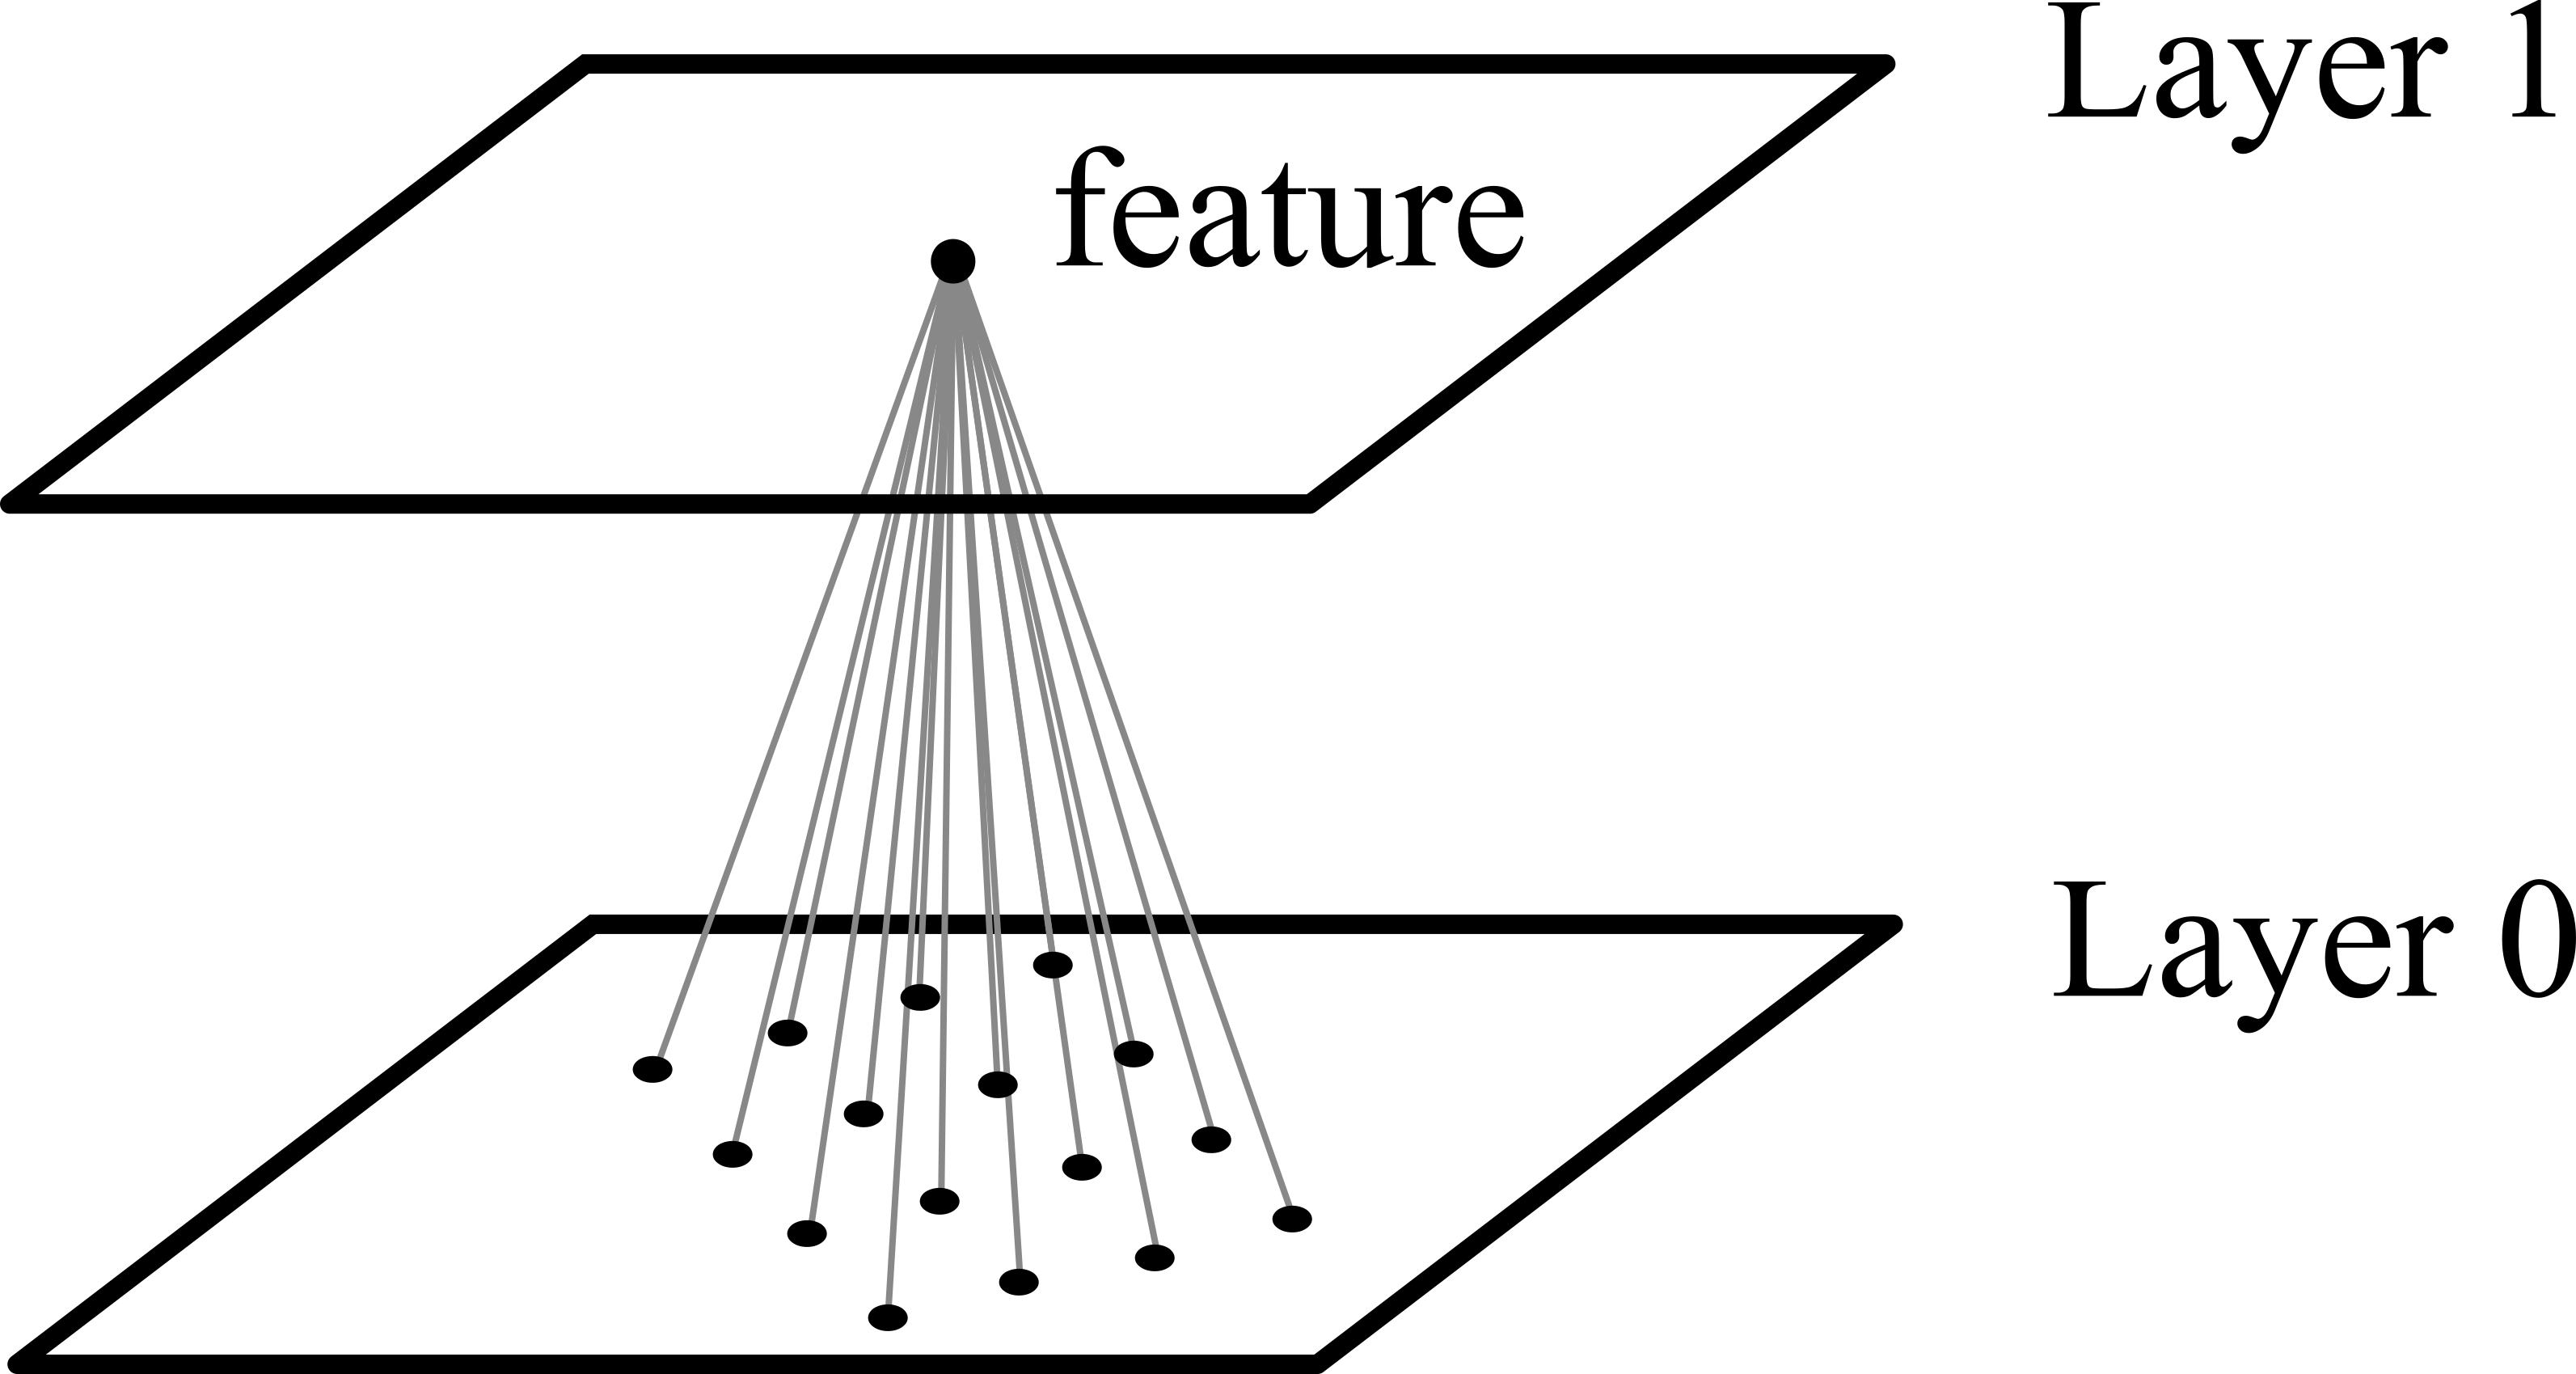
\includegraphics[scale=0.6]{feature.png}}}
\end{equation}

A \textbf{feature} = \textbf{neuron}, is a \textbf{filter} applied to a \textit{local} part of the \textbf{input signal}, usually implemented as a \textbf{dot product} followed by a \textbf{non-linearity} $\sigmoid$:
\begin{equation}
\boxed{\mbox{neuron}} = \boxed{\mbox{feature}} = \sigmoid \; \langle \vect{v}, \vect{w} \rangle .
\end{equation}
Such a function is also called a \textbf{ridge function}.  $\vect{v}$ is the \textbf{input} vector, $\vect{w}$ is the \textbf{weight} vector.

Last time I forgot to mention that the non-linearity $\sigmoid$ being a \textbf{sigmoid} function is not essential to a neural network.  In fact, any non-linearity will do, as long as it is \textit{continuous} and has first-order derivatives.  That even includes \textbf{piecewise-linear} functions.

The ``universal'' approximation ability of neural networks comes from the \textbf{Weierstrass approximation theorem} (1885) that says that every continuous function can be uniformly approximated by polynomials.  This is later generalized to the \textbf{Stone-Weierstrass} theorem (1937).  For neural networks, the universal approximation property can be proven with just a single layer --- which means it does not depend on the ``deep'' property.

If we have a \textbf{pool} of features or neurons, they form a \textbf{layer}:
\begin{equation}
\boxed{\mbox{pool of neurons}} = \boxed{\mbox{layer}} = \sigmoid( \; W \vect{v} \; )
\end{equation}
where $W$ is a \textbf{matrix} of weights.  $\sigmoid$ is applied \textit{component-wise} to the resulting vector.

A deep network is just the \textbf{composition} of many layers:
\begin{equation}
\boxed{\mbox{deep network}} = [ \sigmoid \; W ]^L \;\; \vect{v} .
\end{equation}

\section{Structure of a ConvNet}

In the convolutional network, each \textbf{feature} is replaced by a convolutional feature:
\begin{equation}
\label{eqn:convolution-feature}
\boxed{\mbox{convolutional feature}} = \sigmoid( \; f * g \; )
\end{equation}
where $f, g$ are functions, $f$ is a \textbf{filter} applied to the \textbf{input} $g$.

We can regard the input signal as a \textbf{function} or as a discretized \textbf{vector} of its graph:
\begin{equation}
\vcenter{\hbox{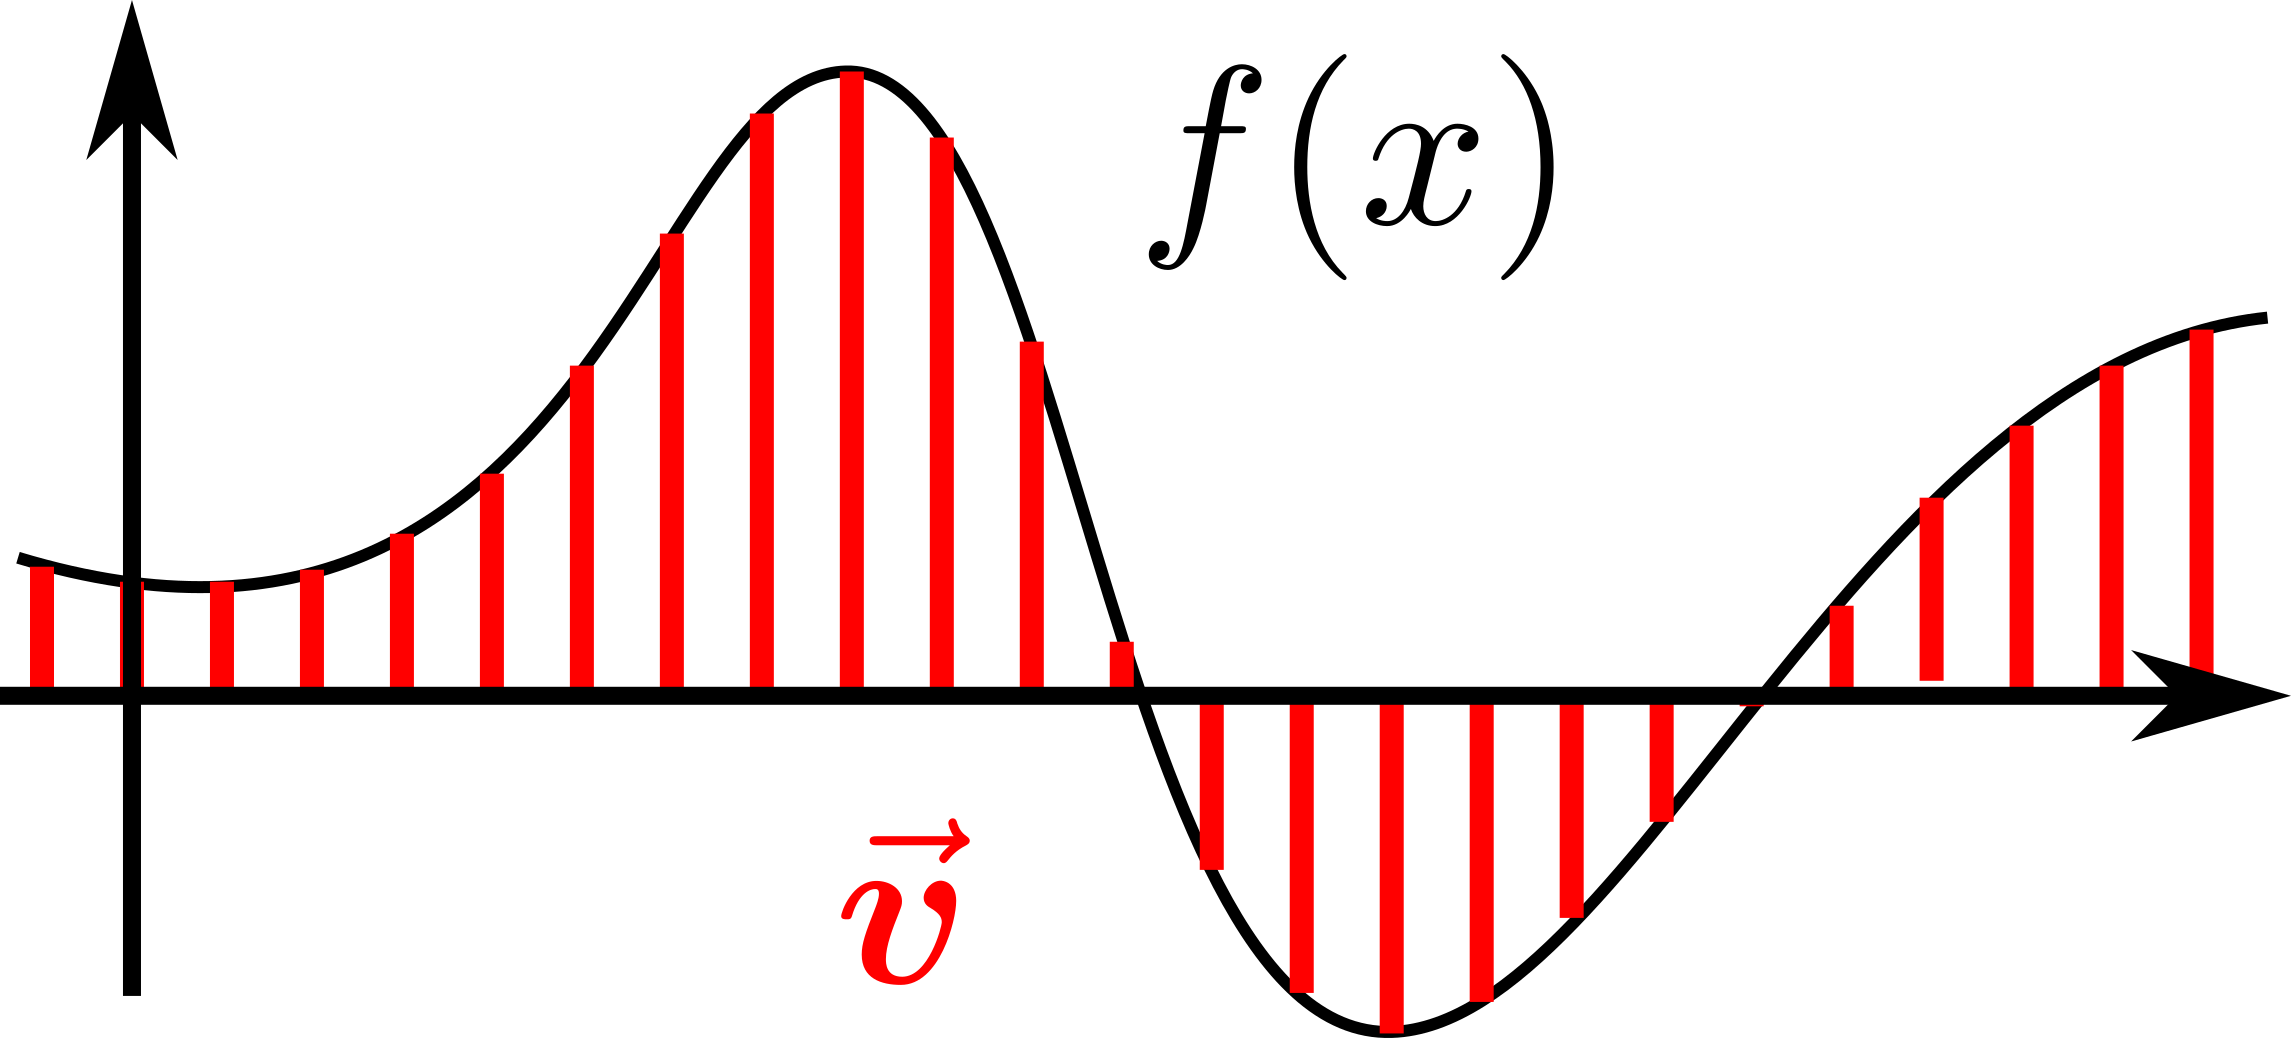
\includegraphics[scale=0.6]{discretized-function.png}}}
\end{equation}
so there is no big difference between a function and a vector, in this context.

When implemented on a computer, the discrete, \textbf{full convolution} is defined as
\footnote{Thanks to 孙小也 at 知乎 (Zhihu.com) for providing these formulas.}:
\begin{equation}
\boxed{\mbox{full convolution}} \quad 
\vect{x} * \vect{k} = \sum_{i = -\infty}^{\infty} \sum_{j = -\infty}^{\infty} \vect{x}_{i j} \; \vect{k}_{u-i, v-j} .
\end{equation}

A \textbf{valid} convolution is a restriction of the full convolution to a \textbf{window}:
\begin{equation}
\boxed{\mbox{valid convolution}} \quad 
\vect{x} * \vect{k} = \sum_{i = -\infty}^{\infty} \sum_{j = -\infty}^{\infty} \vect{x}_{i+u, j+v} \; \vect{k}_{\mathrm{rot} \; i, j} \; \chi(i, j) 
\end{equation}
\begin{equation}
\nonumber
\chi(i, j) = 
\begin{cases}
1, \quad \quad 0 \le i,j \le n \\
0, \quad \quad \mbox{otherwise}
\end{cases}
\end{equation}
where $\vect{k}_{\mathrm{rot}}$ is $\vect{k}$ rotated by $180^\circ$. 

The pool of local features has a lot of \textbf{redundancy}, which can be reduced by \textbf{sub-sampling} them:
\begin{equation}
\boxed{\mbox{sub-sampling}} \quad 
\vect{x}_{i, j}^{(\ell + 1)} = \sigmoid( \; \beta \sum_{u = ir}^{(i+1)r-1} \sum_{v = jr}^{(j+1)r-1} \vect{x}_{u, v}^{(\ell)} \; )
\end{equation}
where $\beta$ is a scalar weight.  The output is a matrix of \textit{reduced} size: $\displaystyle \left( \frac{m-n-1}{r} \times \frac{m-n+1}{r} \right)$.

Repeating this structure gives rise to the following typical architecture (which I won't explain in detail):
\begin{equation}
\vcenter{\hbox{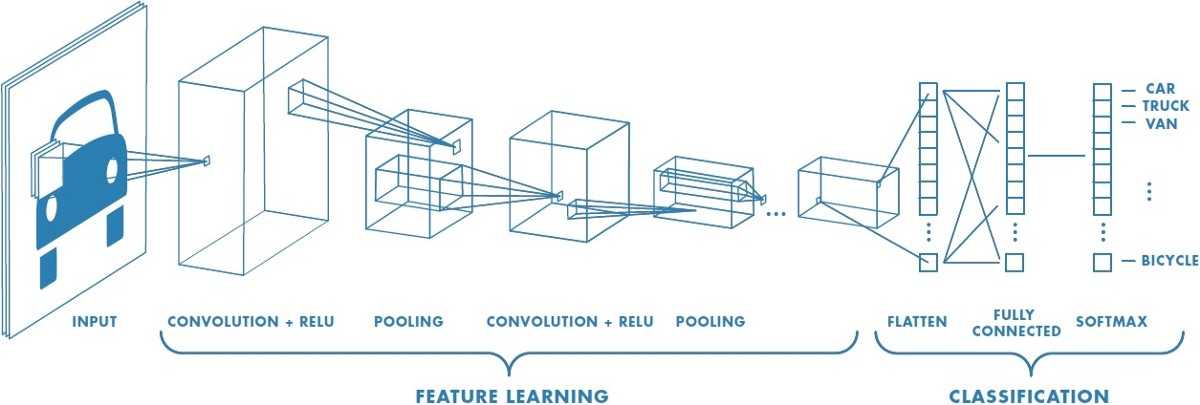
\includegraphics[scale=0.4]{ConvNet-architecture.png}}}
\end{equation}

\section{Symmetric neural networks}

For \textbf{vision}, we need invariance under translations as well as rotations, scaling, etc.  In short, \textbf{affine transformations}.  ConvNet merely provides translational invariance, but the boost in learning speed is sufficient to kick start a revolution in computer vision.

Now we turn to the topic of symbolic \textbf{logic}, my research focus.  Suppose the input is a list of vectors $(\vect{v}_1, \vect{v}_2, ... , \vect{v}_K)$.  We want neural networks that are invariant under \textbf{permutations} of the vectors $\vect{v}_i$; in other words, invariant under the action of the symmetric group $\mathfrak{S}_K$.

Such a requirement would impose some constraints on the weights of the neural network.  For a long time, I thought it would be impossible to realize such constraints in a neural network, but I wasn't aware that the other researchers have investigated the problem and gotten significant results.  For example Domingos and Gens's 2014 idea
\footnote{Robert Gens and Pedro Domingos 2014, \textit{Deep symmetry networks}, NIPS'14, proceedings of the 27th international conference on Neural Information Processing Systems, v2, 2537-2545.}.

Note that Pedro Domingos also has a research interest in logic-based learning (with neural networks), and he is the author of the book \textit{The Master Algorithm: How the Quest for the Ultimate Learning Machine Will Remake Our World}.
\begin{equation}
\nonumber
\vcenter{\hbox{
\includegraphics[scale=0.5]{Pedro-Domingos.jpg}}}
\end{equation}

Their idea is simply to replace the convolution operator in (\ref{eqn:convolution-feature}) with other \textbf{filters} that have desired invariance properties (\textit{eg} affine invariance).  The resulting neural network is training with back-propagation as usual.

So perhaps we can use the following kind of features for the logical purpose:
\begin{equation}
\label{eqn:commutative-feature}
\boxed{\mbox{commutative feature}} = P_{\mathrm{sym}} (\vect{v}_1, \vect{v}_2, ..., \vect{v}_n)
\end{equation}
where $P_{\mathrm{sym}}$ is a \textbf{symmetric polynomial} (which is already non-linear so we don't need the $\sigmoid$ function).

So we have the following correspondence:
\begin{equation}
\begin{tabular}{|l|l|l|l|}
	\hline
	levels: & \textbf{neurons} = features & \textbf{pool} = layer & \textbf{network} \\
	\hline
	\textbf{neural networks} & \parbox[t]{5cm}{dot product \\ $\sigmoid \; \langle \vect{v}, \vect{w} \rangle$ } & matrix & composition of layers \\[1.5em]
	\hline
	\textbf{ConvNets} & \parbox[t]{5cm}{convolution \\ $\sigmoid( \; f * g \; )$ } & pool & composition of layers \\[1.5em]
	\hline
	\textbf{SymNets} & \parbox[t]{5cm}{symmetric polynomials \\ $P_{\mathrm{sym}} (\vect{v}_1, \vect{v}_2, ..., \vect{v}_n)$ } & pool & composition of layers \\[1.5em]
	\hline
\end{tabular}
\end{equation}

Unfortunately, if $P_{1234}$ is symmetric over $(\vect{v}_1,...,\vect{v}_4)$, and $P_{5678}$ symmetric over $(\vect{v}_5,...,\vect{v}_8)$, then $P_{1234} + P_{5678}$ may not be invariant if we swap $\vect{v}_1$ with $\vect{v}_5$, say.

First consider the simple case where the vectors $\vect{v}_i$ are 1-dimensional.  

\end{document}
